\documentclass{article}
\usepackage[utf8]{inputenc}
\usepackage{authblk}
\usepackage{setspace}
\usepackage[margin=1.25in]{geometry}
\usepackage{graphicx}
\graphicspath{ {./Plots/} {./figures/} }
\usepackage{subcaption}
\usepackage{amsmath}
\usepackage{lineno}
\linenumbers
\usepackage{algorithm}
\usepackage{algpseudocode}
\usepackage{textcomp} % For proper R\textsuperscript{2} symbol
\usepackage[style=numeric, 
citestyle=numeric-comp,
sorting=none]{biblatex}  % Changed from nejm to numeric
\addbibresource{Unsupervised_plant_counting.bib}
\usepackage{url}

%%%%%% Title %%%%%%
\title{On the minimum dataset requirements to fine-tune an object detector for arable crops plant counting: A downstream case study on maize seedlings}

%%%%%% Authors %%%%%%
\author[1*]{Samuele Bumbaca}
\author[1]{Enrico Borgogno-Mondino}

%%%%%% Affiliations %%%%%%
\affil[1]{Department of Agricultural, Forest and Food Sciences, University of Turin, 10095 Grugliasco, Italy}
\affil[*]{Address correspondence to: samuele.bumbaca@unito.it}

%%%%%% Date %%%%%%
\date{}

%%%%%% Spacing %%%%%%
\onehalfspacing

\begin{document}

\maketitle

%%%%%% Abstract %%%%%%
\begin{abstract}
Effective object detection in precision agriculture requires understanding 
minimum dataset requirements, yet this remains undetermined for arable crops seedling detection. 
This study investigates the minimum dataset size and quality needed to achieve benchmark 
performance (R\textsuperscript{2} = 0.85) across different object detection paradigms. We systematically 
evaluated many-shot models (YOLOv5, YOLOv8, YOLO11, RT-DETR), few-shot (CD-ViTO), 
and zero-shot (OWLv2) approaches using orthomosaic imagery of maize seedlings, while 
also implementing a handcrafted algorithm as baseline. Models were tested with varying 
dataset sizes, quality levels, and training sources (in-domain vs out-of-distribution). 
Results demonstrate that no out-of-distribution trained model achieved benchmark 
performance, while in-domain trained models reached the benchmark with 60-130 annotated 
images, depending on architecture. Transformer-mixed models (RT-DETR) required fewer 
samples (60) than CNN-based models (110-130), but showed different sensitivities 
to annotation quality reduction. Models maintained benchmark performance with 65-90\% 
of original annotation quality. Neither few-shot nor zero-shot approaches met benchmark 
requirements despite their recent advances. These findings provide practical guidance 
for efficiently developing maize seedling detection systems, emphasizing that successful 
deployment requires in-domain training data, with minimum requirements dependent 
on model architecture.
\end{abstract}

%%%%%% Main Text %%%%%%

\section{Introduction}

\subsection*{The Problem of Plant Counting}

Plant counting is a critical operation in precision agriculture, plant breeding, 
and agronomical evaluation. 
Accurate plant counts can provide valuable information for both farmers and researchers.
This task was often performed manually by human operators. 
Today, this process can be automated by the use of computer vision algorithms.
To validate a method for counting, it is critical to set a benchmark for accuracy. 
A benchmark can be defined by the accuracy of manual counting, international standards, 
or by comparison with other already accepted methods.
Accuracy of plant manual counting depends on human performance, so variable, but often taken as golden sample. 
According to the European Plant Protection Organization, the benchmark for acceptance is 
a coefficient of determination (R\textsuperscript{2}) of 0.85 when compared to manual counting \cite{PP13332024}.
This corresponds to a Root Mean Square Error (RMSE) of approximately 0.39.
Also scientific literature mention a R\textsuperscript{2} value of 0.85 with ground truth (manual counting) 
as a benchmark for acceptance \cite{zouMaizeTasselsDetection2020}.

Literature shows that benchmark for acceptance can be achieved with computer vision object detection
\cite{liuIntegrateNetDeepLearning2022,davidPlantDetectionCounting2021,barretoAutomaticUAVbasedCounting2021}
or regression models \cite{liuEstimatingMaizeSeedling2022,EstimatesMaizePlant}.
A superiority of object detection over regression models in terms of accuracy was found
\cite{zouMaizeTasselsDetection2020}. Object detection is also more versatile than
regression models, because, object detection model inference on georeferenced orthomosaics delivers 
plants geographical coordinates, not only density per area.
The validation of this ability rely on metrics as Intersection over Union ($IoU$),
Average Precision (AP), and Average Recall \cite{linMicrosoftCOCOCommon2015} rather than
the coefficient of determination. 
Identification supports are usually bounding boxes, which are rectangles that enclose
the object of interest, but they can also be points or other kind of geometries.
Counting of plants is then commonly performed by counting the number of geometries 
that enclose the objects of interest (the plant) in a image area.
Georeferenced orthomosaics are images created through aerial photogrammetry, a process 
that involves capturing overlapping georeferenced images taken by nadiral view 
picturing georeferenced ground control points, and performing bundle adjustment to form 
a single, seamless image \cite{krausPhotogrammetryGeometryImages2011}.
Georeferenced orthomosaics are scaled and oriented to a geographical coordinate system.
It implies that the pixel coordinates corresponds to 
geographical coordinates and are projectables in a metric system.
Using georeferenced orthomosaics in seedling counting makes object detection 
easier, because the metric scale can be used to locate the objects 
in the image and prospective variance is reduced to zero.

\subsection*{Case study: Maize Seedling Counting}

Plant counting is affected, as many object detection application fields, from data scarcity: public datasets
are rare and often not suitable for the task because of the large environmental
variability and their images are not orthorectified or scale is unknown. 
Even so, some useful dataset for training a plant counting object detector can be found in public repositories \cite{heiderSurveyDatasetsComputer2025}.
These dataset may come as a part of a scientific study or with poor technical specifications. 
Selecting a specific crop at a specific growth stage can reduce the variability that 
the model should learn and make it possible to better study the other variables
that can affect the dataset size and quality requirements. 
For this study we choose grain maize seedlings
(Zea mays L.) at the V3-V5 (BBCH 13-15) growth stage \cite{meierBBCHSystemCoding2009},
because it is the most represented plant in scientific \cite{davidPlantDetectionCounting2021,liuIntegrateNetDeepLearning2022}
and not scientific \cite{Maize_seedingDatasetOverview,MaizeseedlingdetectionDatasetOverview}
open datasets from aerial photogrammetry. 
Maize is a commodity crop that is widely grown in the world and is the most important
crop in the world by production \cite{fao2024}. Grain maize seedlings in that stage are easy to
count because of their low overlapping and fixed intra-row and inter-row spacing, 
differently by silo-maize seedling that is seeded with extremely low inter-row spacing.
This particular seedling configuration that makes grain maize a good candidate for object detection,
is shared with other crops that are seeded in rows with inter-row spacing such as sunflower (Helianthus annuus L.)
or sugarbeet (Beta vulgaris L.).

\subsection*{Object Detection approaches}

The development of object detection algorithms has evolved from not machine learning methods, 
here named handcrafted methods (HC), to modern deep learning-based (DL) techniques.
Today, all the state-of-the-art object detection methods are based on DL models. 
Nevertheless, HC methods are still used in some cases 
\cite{davidPlantDetectionCounting2021,garcia-martinezDigitalCountCorn2020}. 
Most of modern DL object detection uses convolutional neural networks (CNN) \cite{lecunDeepLearning2015} based 
frameworks (e.g., Faster R-CNN \cite{FasterRCNNRealTime}, YOLO \cite{YouOnlyLook}) 
or Transformer \cite{vaswaniAttentionAllYou2017} based approaches (e.g., DETR \cite{carionEndtoEndObjectDetection2020})
or mixtures of both approaches.
The main difference between CNN-based and Transformer-based models is the way they
process the image. CNN-based models process the image in a grid-like fashion (convolutions),
while Transformer-based models process the image as a sequence of patches (attention mechanisms) \cite{dosovitskiyImageWorth16x162021}.
On common benchmarks as COCO \cite{linMicrosoftCOCOCommon2015}, PASCAL VOC \cite{jingSelfsupervisedVisualFeature2019}, 
and ImageNet \cite{14090575ImageNetLarge}, Transformer-based models have shown 
to be more accurate than CNN-based models \cite{zongDETRsCollaborativeHybrid2023}.
CNN-based models are still widely used in object detection, because they are
more efficient in processing small images and have a lower computational cost \cite{khanSurveyVisionTransformers2023}.
However, when fine-tuning with scarce data, Transformer-based object detectors generally 
perform better than CNN-based detectors, provided they are pretrained on large datasets \cite{rekavandiTransformersSmallObject2023,liTransformerObjectDetection2023,amjoudObjectDetectionUsing2023}.

To represent the categories and compare performance between pure-CNN and Transformer-mixed architectures
that are effectively used as object detectors in real plant counting applications,
YOLOv5 and YOLOv8 can be taken as pure-CNN architecture representatives for their 
large use in agriculture \cite{badgujarAgriculturalObjectDetection2024}.
Their large diffusion in agriculture applications is justified by the fact that they leverage good precision
and the low need in terms of dataset size in respect other CNN architectures \cite{tanEfficientDetScalableEfficient2020,linFocalLossDense2018,zhangComparisonYOLObasedSorghum2025}.

Real-Time-DETR (RT-DETR) is a recent Transformer-mixed architecture that outperforms
YOLOv5 and YOLOv8 \cite{zhaoDETRsBeatYOLOs2024}. 
YOLO11 has been recently proposed as a
Transformer-mixed YOLO architecture that outperforms RT-DETR on COCO dataset \cite{khanamYOLOv11OverviewKey2024}.

Recently, zero-shot and few-shot object detection have emerged as promising paradigms
to alleviate the need for large annotated datasets.
While traditional object detection models (many-shots object detectors) require extensive labeled data for training, 
few-shot and zero-shot object detection aim to detect novel objects with little to 
no labeled examples respectively. The term "shot" refers to the number of annotations 
used to train the model over all the images. Each shot corresponds to an individual, 
that in the case of few-shots, is used to prototype the object of interest.
Zero and few-shots approaches often leverage feature transfer or meta-learning components to generalize 
across classes under extreme data scarcity \cite{liMetaSGDLearningLearn2017}. This approach reduces the annotation 
burden and is especially beneficial in domains where collecting exhaustive training 
data is impractical.
Zero-shot object detection detects new categories without any training samples by 
leveraging semantic relationships or contextual information learned from known classes \cite{bansalZeroShotObjectDetection2018}. 
Few-shot approaches optimize models to learn quickly from a handful of labeled examples \cite{huangSurveySelfSupervisedFewShot2022}.
Meta learning is a common approach in few-shot object detection 
\cite{MetaLearningBasedIncrementalFewShot,wuMetaRCNNMetaLearning2020,fuMetaSSDFastAdaptation2019,zhangMetaDETRFewShotObject2021}, 
while Cross-Domain Few-Shot Object Detection (CD-FSOD) has recently surpassed this
approach by leveraging domain adaptation techniques \cite{saBroaderStudyCrossdomain2023}.
DE-ViT \cite{xuDeViTDecomposingVision2023} and CD-ViTO \cite{fuCrossDomainFewShotObject2024}  
are the latest models that have shown promising results in few-shot object detection.

Zero-shot actual state-of-the-art object detector models are YOLO-World \cite{kangFewshotObjectDetection2019}, 
OWLv2 \cite{mindererScalingOpenVocabularyObject2023}, and Grounding DINO \cite{liuGroundingDINOMarrying2025}.
OWLv2 (Open-World Localization v2) is an zero-shot object detector that represented a significant 
evolution in open-vocabulary detection capabilities.

\subsection*{Dataset Size and Quality Requirements}

As already mentioned, the performance comparison between object detection models is
usually based on differences in metrics such as AP, calculated on standard datasets
that are not representative of the agricultural application field.
Many studies have been conducted on object detection for plants in open field
\cite{barretoAutomaticUAVbasedCounting2021,gengResearchSegmentationMethod2024,jiangDeepSeedlingDeepConvolutional2019,katariIntegratingAutomatedLabeling2024,kitanoCornPlantCounting2019,liDCYOLOImprovedField2024,liSeedlingMaizeCounting2022,liuIntegrateNetDeepLearning2022,liuEstimatingMaizeSeedling2022,luTasselNetCountingMaize2017,macheferMaskRCNNRefitting2020,velumaniEstimatesMaizePlant2021,wangPlotLevelMaizeEarly2023,zhaoStudyLightweightModel2023},
but few have argued or focused on dataset minimum requirements for training a robust plant object detector
\cite{davidPlantDetectionCounting2021,andvaagCountingCanolaGeneralizable2024}.
Some study focused on few-shots approach for plant counting \cite{wangPlotLevelMaizeEarly2023,amirkolaeeAdaTreeFormerFewShot2024},
but only two specifically accounting on few-shots method for maize seedling counting \cite{karamiAutomaticPlantCounting2020,wangAdvancingImageRecognition2024}.
Unfortunately, the lonely two studies evaluating few-shot performance on maize seedling counting 
by orthomosaics do not achieve the benchmark and do not clearly
specify the number of shots used. Also no zero-shot benchmark for maize seedling counting 
has been set yet, and no research on this application has been done yet.

This critical research gap presents significant challenges for practitioners in precision agriculture 
who must decide how much data to collect and annotate for effective maize seedling detection. Without 
systematic evaluation of minimum dataset requirements across different detection approaches (many-shot, 
few-shot, and zero-shot), it remains unclear whether resource-intensive manual annotation can be 
reduced or eliminated. Furthermore, the agricultural domain's unique characteristics: variable environment, 
and plant phenotype, may fundamentally alter the data requirements 
compared to general computer vision benchmarks. Determining these requirements would provide practical 
guidance for implementing object detection in agricultural workflows while optimizing the trade-off between 
annotation effort and detection performance.

Even if no research has been made in order to minimize or set a benchmark for the dataset size and quality
required to train a maize seedling object detector,
it is well known that the performance of a DL model is directly related to the
amount of data used for training \cite{sunRevisitingUnreasonableEffectiveness2017} and 
its quality \cite{alhazmiEffectsAnnotationQuality2021}.
Dataset size and quality predictability in DL has been proven to be
addressable with empirical approaches \cite{hestnessDeepLearningScaling2017,mahmoodHowMuchMore2022}.
As already mentioned, model architecture is critical in dataset requirements as different models may require
different dataset sizes and qualities to achieve the same performance \cite{nguyenEvaluationDeepLearning2020,brigatoCloseLookDeep2020}.
Backbone is pivotal on downstream tasks as object detection \cite{duSpineNetLearningScalePermuted2020}. 
The importance of using a domain specific backbone has been proven also
for plant/leaves segmentation on orthomosaics \cite{roggiolaniDomainSpecificPreTraining2023},
but backbone training is still prohibitive for many applications.
No backbone weights specialized on agricultural orthomosaics has been published yet,
as for the most of the specialized domains. Even if a so specialized backbone exists,
some concern will came out about its out-of-distribution generalization capability \cite{hendrycksManyFacesRobustness2020}.
So, because of limited resources, today only the use of a general backbone is 
possible in practical sense \cite{jeevanWhichBackboneUse2024},
even if a decreasing in dataset size requirements is expected with a domain specific 
backbone because of the out-of-distribution generalization \cite{goldblumBattleBackbonesLargeScale2023}.
Another factor that can affect the dataset size and quality requirements other than 
the already cited model architecture and use of pre-trained backbones, is the training data
augmentation strategy. Some studies proposed hightly computationally expensive data augmentation
such as trainable data augmentation \cite{cubukAutoAugmentLearningAugmentation2019} or
data augmentation with generative adversarial networks \cite{antoniouDataAugmentationGenerative2018}.
Other studies proposed to use less computationally expensive data augmentation strategies
\cite{shortenSurveyImageData2019,chadebecDataAugmentationVariational2021} and someone
even proved that random image augmentation can provide equivalent results to more
expensive technics \cite{mullerTrivialAugmentTuningfreeStateoftheArt2021}.
As also image augmentation can lead to prohibitive computational costs, the use of
less computationally expensive data augmentation strategies is recommended for
fine-tuning to downstream tasks \cite{shortenSurveyImageData2019}.

Nevertheless, the most important factor affecting DL training is the dataset source 
\cite{sunRevisitingUnreasonableEffectiveness2017}. 
It has been observed that using training samples from the same
dataset as the inference (in-domain dataset) dramatically increases accuracy and reduce the need 
for a large dataset in respect to collecting training samples from other 
datasets (out-of-distribution dataset) \cite{davidPlantDetectionCounting2021,andvaagCountingCanolaGeneralizable2024}. 
From comparison of the studies here mentioned, dataset source seems to be the most 
important factor in determining the dataset size and quality needed to achieve the benchmark 
for acceptance.

\subsection*{Study Aim}

This study aims to determine the minimum dataset size and quality required to train 
a object detection model for identifying maize seedlings in georeferenced orthomosaics
achieving the benchmarks set by international organizations and recognized in scientific literature.
Here, the dataset size and quality are respectively defined as the amount of annotated 
images in the training set, and the accuracy of the annotations.
Also the effect of training dataset source will be evaluated in this study.
Models architecture and size will be taken into account, as long as the object detection
downstream task is concerned. 
After setting the dataset size and quality minimum requirements for many-shots
object detectors, we will evaluate if new zero-shot and few-shot object detection
models can achieve the same benchmark for acceptance with less data and annotations.
We will also discuss the need for HC method in a DL object detection pipeline.

%%%%%%%%%%%%%%%%%%%%%%%%%%%%%%%%%%%%%%%%%%
\section{Materials and Methods}

\subsection{Experimental Design}
This study investigated the minimum dataset size and quality requirements for training object detection models to count maize seedlings in georeferenced orthomosaic images. We conducted a systematic evaluation across three object detection paradigms:
\begin{itemize}
    \item Many-shot models (YOLOv5, YOLOv8, YOLO11, RT-DETR) trained with varying dataset sizes (10-150 images)
    \item Few-shot models (CD-ViTO with ViT backbones) trained with 1-50 shots
    \item Zero-shot models (OWLv2) using various text prompts without training
\end{itemize}

Each model was evaluated against the benchmark performance threshold of R\textsuperscript{2} = 0.85 for plant counting accuracy. We further analyzed how dataset source (in-domain vs. out-of-distribution) and annotation quality (10-100\%) affected model performance.

\subsection{Datasets}
The datasets used in this study to train the object detection models for maize seedlings
counting are nadiral or supposedly nadiral images of maize seedlings at the V3-V5 growth stage
or estimated so.
The V3-V5 growth stage is defined by the BBCH scale as the stage where the third to fifth
leaf is unfolded and the plant is 15-30 cm tall \cite{meierBBCHSystemCoding2009}.

This study uses two dataset sources as training sets: the out-of-distribution dataset (OOD)
and the in-domain dataset (ID). The ID datasets are from the same source as the
testing dataset, while the OOD datasets are not.
The OOD datasets are composed of images from scientific literature \cite{liuEstimatingMaizeSeedling2022,davidPlantDetectionCounting2021}
and from internet repositories \cite{Maize_seedingDatasetOverview,MaizeseedlingdetectionDatasetOverview}.
The ID datasets were collected during this study. This ID dataset creation consisted in
capturing nadiral images of three study areas with a Phantom 4 Pro v2.0 (DJI, Shenzhen, China)
drone equipped with its default series RGB camera @ ~10 m AGL (above the ground level).
The number of images captured depends on the study area size that was about 2 hectares
for ID\_1 location and about 1 ha for the other two.
For each location, an orthomosaic was created using a photogrammetric software.
Bundle adjustment error was estimated as 38 mm using the ground control points
surveyed by GNSS operating in VRS-NRTK mode. The orthomosaics were generated with an 
average ground sampling distance of 5 mm/pixel in the WGS84/UTM 32 N reference system.

The OOD scientific datasets consist of tiles of georeferenced orthomosaics of maize seedlings from scientific literature.
The OOD internet datasets consist of RGB images of maize seedlings from internet repositories.
The ID datasets were collected during this study and consist of tiles of georeferenced orthomosaics of maize seedlings of known scale.
The OOD scientific datasets and the ID datasets are composed of tiles of georeferenced orthomosaics 
of known scale, while the OOD internet datasets are simple RGB images of unknown scale.
All the OOD datasets came with annotations, while the ID datasets were manually annotated.
The OOD dataset annotation are rectangular bounding boxes centering on an individual plant stem.
ID dataset annotation was done during this study by an agronomist by observing the 
entire orthomosaic on a Geographical Information System (GIS) environment, 
with the tiles grid overlapping the orthomosaic to focus on target tiles without losing the surrounding
context, so without losing bordering plants. Annotations were created as squared 
bounding boxes of size length equal to the minimum distance between two plants in the row, 
with each box centered on an individual seedling stem. 

\begin{table}[h]
\caption{Summary of Datasets Used in the Study}
\label{tab:datasets}
\centering
\begin{tabular}{lccccc}
\hline
\textbf{Dataset} & \textbf{Phenological Stage} & \textbf{Train Size} & \textbf{Test Size} & \textbf{RGB mean} & \textbf{RGB std} \\
\hline
\multicolumn{6}{l}{OOD Scientific} \\
DavidEtAl.2021 \cite{davidPlantDetectionCounting2021} & V3 & 182 tiles & N/A & [0.53, 0.47, 0.37] & [0.11, 0.11, 0.09] \\
LiuEtAl.2022 \cite{liuEstimatingMaizeSeedling2022} & V3 & 596 tiles & N/A & [0.34, 0.31, 0.29] & [0.34, 0.31, 0.29] \\
\hline
\multicolumn{6}{l}{OOD Internet} \\
OOD\_int\_1 \cite{Maize_seedingDatasetOverview} & V3 & 216 tiles & N/A & [0.51, 0.51, 0.5] & [0.15, 0.16, 0.14] \\
OOD\_int\_2 \cite{MaizeseedlingdetectionDatasetOverview} & V5 & 174 tiles & N/A & [0.43, 0.44, 0.43] & [0.14, 0.15, 0.14] \\
\hline
\multicolumn{6}{l}{ID} \\
ID\_1 & V3 & 150 tiles & 20 tiles & [0.81, 0.64, 0.35] & [0.1, 0.11, 0.11] \\
ID\_2 & V3 & 150 tiles & 20 tiles & [0.67, 0.64, 0.63] & [0.13, 0.13, 0.11] \\
ID\_3 & V5 & 150 tiles & 20 tiles & [0.67, 0.66, 0.65] & [0.14, 0.13, 0.14] \\
\hline
\end{tabular}
\end{table}

\begin{figure}[h]
  \centering
  \begin{subfigure}{0.22\textwidth}
    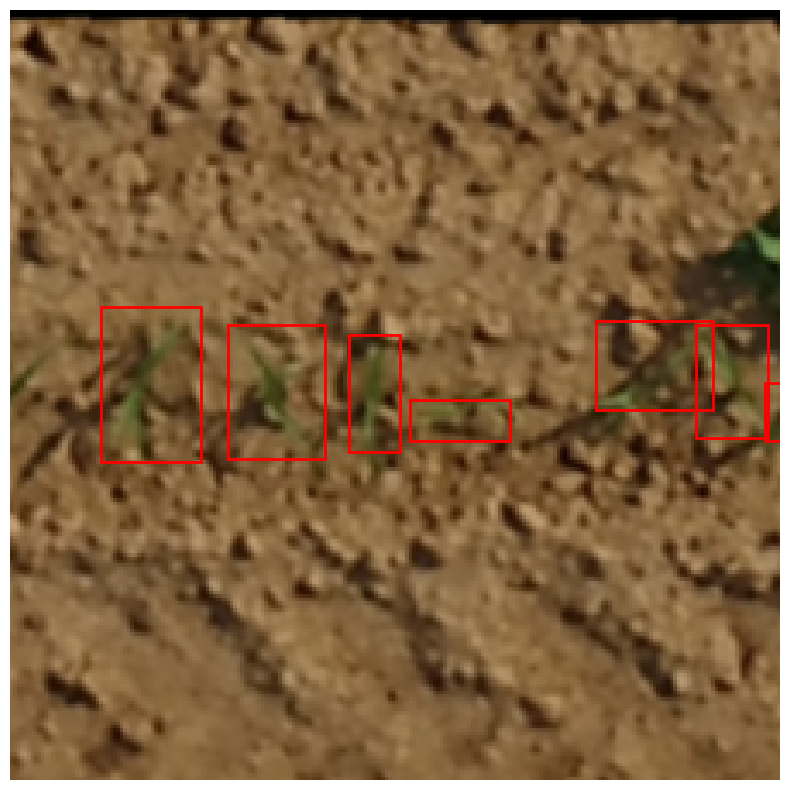
\includegraphics[width=\linewidth]{DavidEtAl.png}
    \caption{}
  \end{subfigure}
  \begin{subfigure}{0.22\textwidth}
    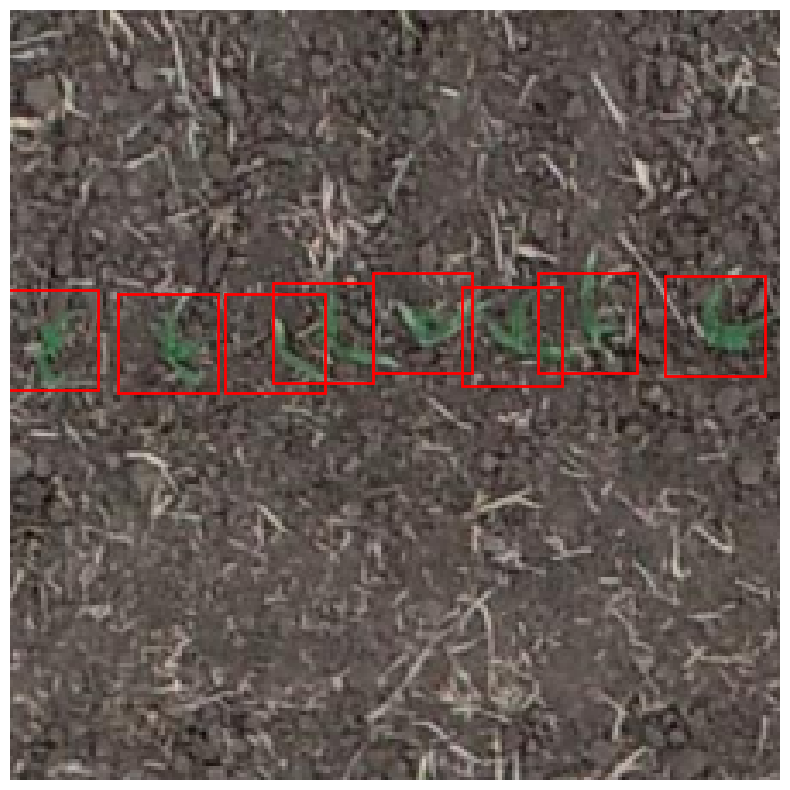
\includegraphics[width=\linewidth]{LiuEtAl.png}
    \caption{}
  \end{subfigure}
  \begin{subfigure}{0.22\textwidth}
    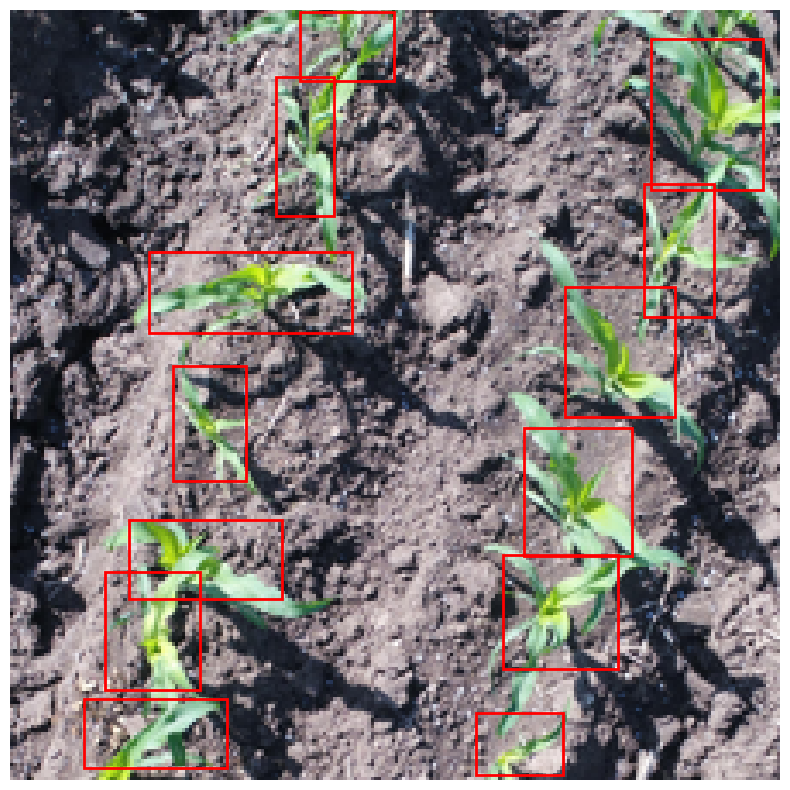
\includegraphics[width=\linewidth]{maize_seedling.png}
    \caption{}
  \end{subfigure}
  \begin{subfigure}{0.22\textwidth}
    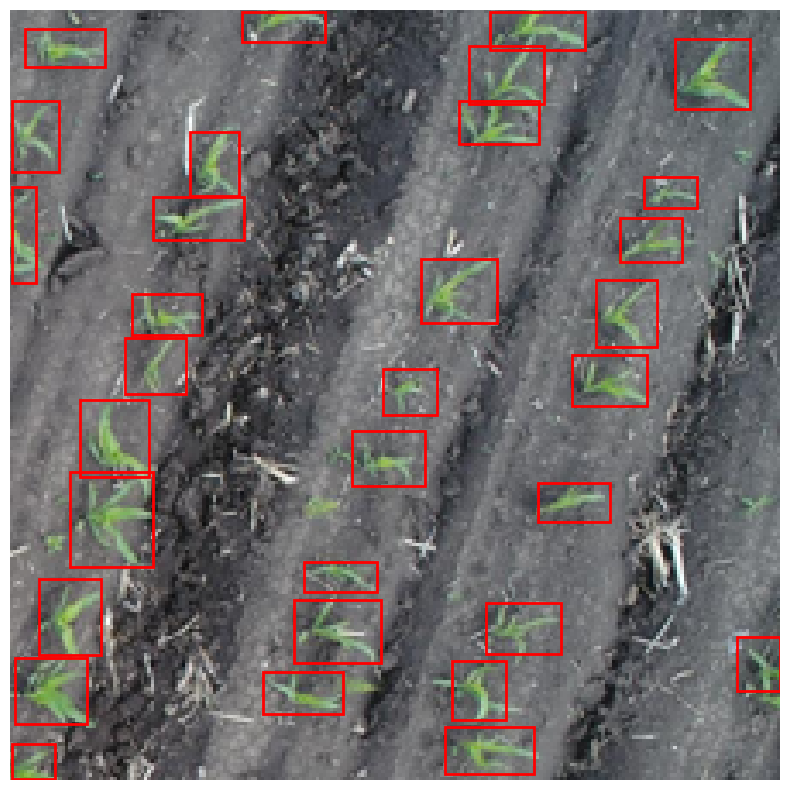
\includegraphics[width=\linewidth]{maize_seedling_detection.png}
    \caption{}
  \end{subfigure}

  \begin{subfigure}{0.3\textwidth}
    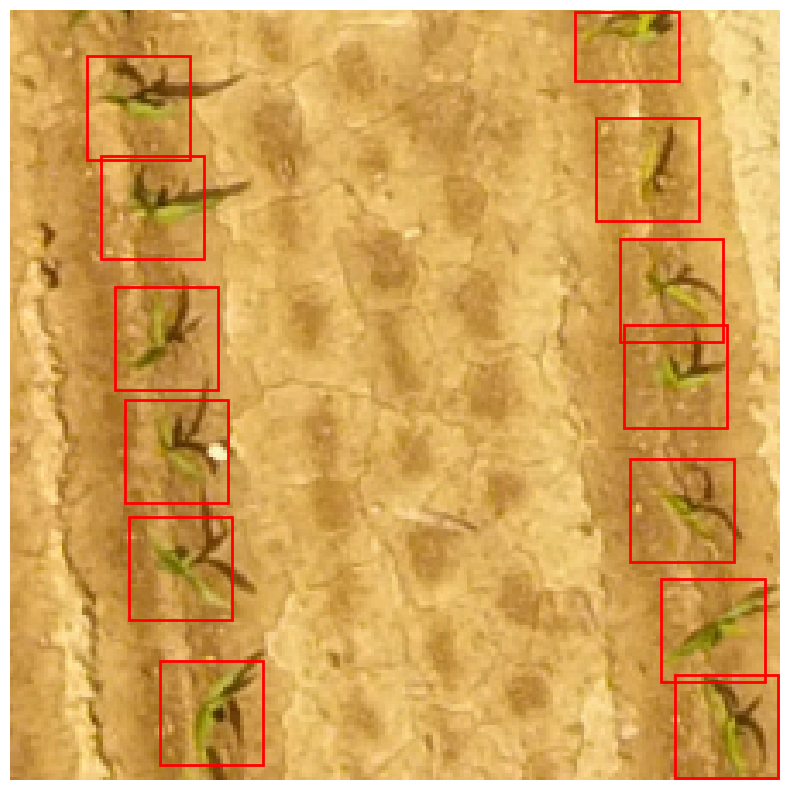
\includegraphics[width=\linewidth]{ID_1.png}
    \caption{}
  \end{subfigure}
  \begin{subfigure}{0.3\textwidth}
    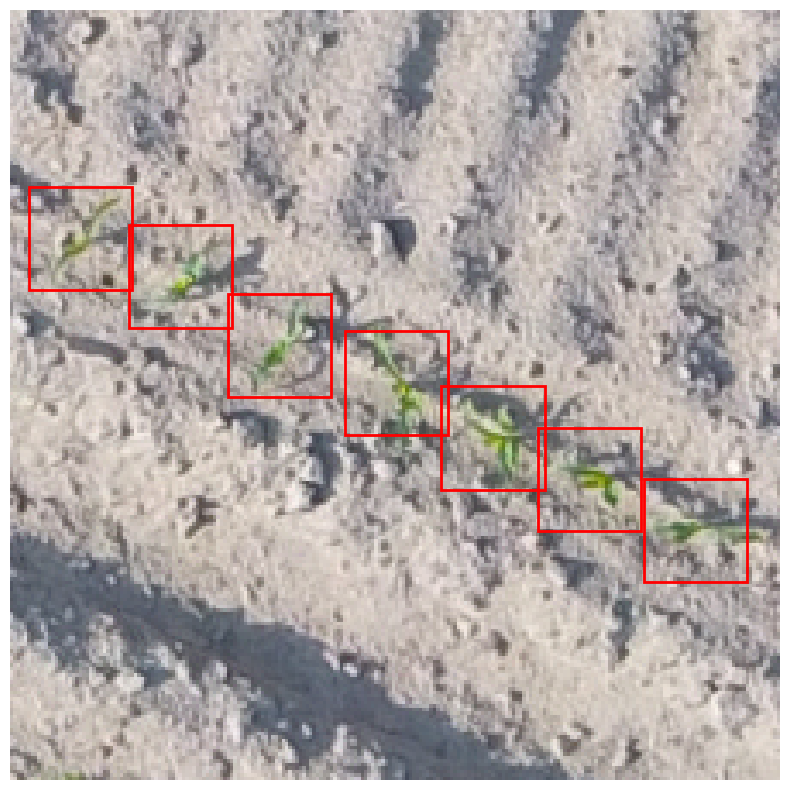
\includegraphics[width=\linewidth]{ID_2.png}
    \caption{}
  \end{subfigure}
  \begin{subfigure}{0.3\textwidth}
    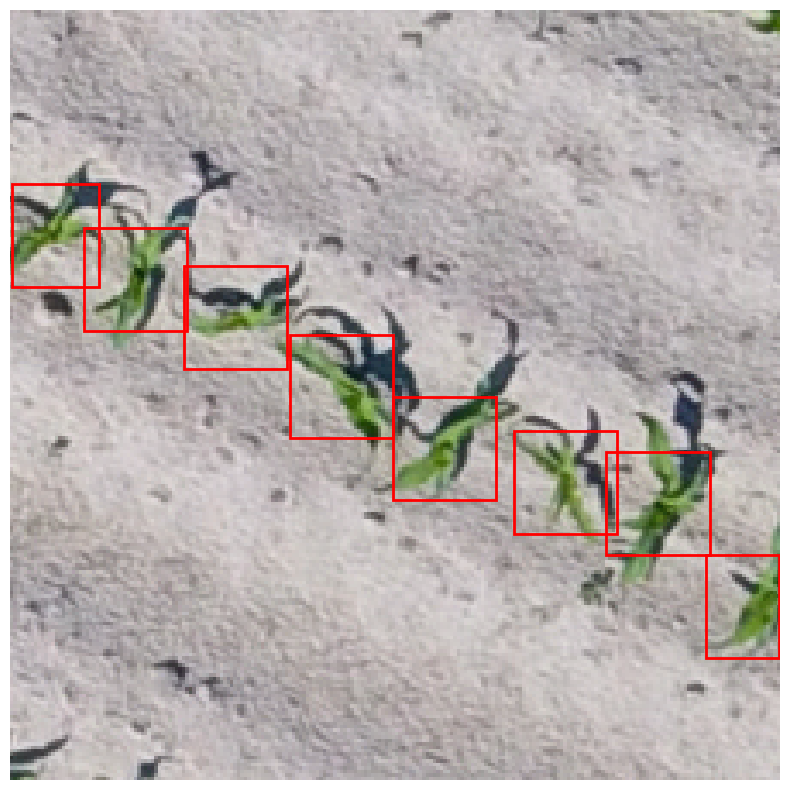
\includegraphics[width=\linewidth]{ID_3.png}
    \caption{}
  \end{subfigure}
  \caption{Dataset examples. (\textbf{a}) DavidEtAl.2021,
  (\textbf{b}) LiuEtAl.2022, 
  (\textbf{c}) Internet Maize stage V3,
  (\textbf{d}) Internet Maize stage V5,
  (\textbf{e}) ID\_1,
  (\textbf{f}) ID\_2,
  (\textbf{g}) ID\_3.}
  \label{fig:datasets}  
\end{figure}

To make the two kind of dataset comparables we chose to rescale the images to a scale of 0.005 m/pixel
where the scale was known (scientific OOD and ID datasets), obtaining orthomosaics of different sizes.
All the orthomosaics were then cropped to 224*224 pixels tiles.
This tile size was selected because at 5 mm/pixel resolution it covers 1.12×1.12 meters of field area.
Given that typical grain maize inter-row distance is 0.75 meters, this size enables capturing 
approximately two rows per tile, which is optimal for row pattern identification in the HC algorithm 
and provides sufficient context for object detection models.
This particular image size was also chosen as a standard from AlexNet \cite{krizhevskyImageNetClassificationDeep2012}
as it should be compatible with most of the object detection architectures.
The annotations were rescaled and cropped where needed.
Figure \ref{fig:datasets} shows a sample for each dataset.
Each ID dataset has 20 tiles to be used as testing dataset, while other 
150 tiles are used as training dataset.

\subsection{Handcrafted object detector}

Like other works \cite{davidPlantDetectionCounting2021,garcia-martinezDigitalCountCorn2020,liuEstimatingMaizeSeedling2022} 
we wrote an HC algorithm to get annotated tiles from the orthomosaics, 
basing it on agronomical knowledge and color thresholding.
Hue, saturation and value (HSV) color space was used here to threshold the image,
to get green pixels, but other color spaces can be used.
For the execution of this algorithm, the following graphical and agronomical 
parameters must be set: color minimum and maximum thresholds (color threshold), the minimum and maximum 
leaf area for plant (leaf area range), the minimum distance between plants on rows (intra-row distance),
and the distance between rows (inter-rows distance). 
The algorithm is expected to works: on orthomosaics of maize seedlings at the V3-V5 growth stage,
with low weeds infestation, with rows having roughly the same angle with meridian and distance between them.

The algorithm is divided in two sequential parts that form a detection-verification pipeline. The first part,
named HC1, performs initial plant detection by thresholding pixels within the specified color range, 
identifying connected regions, and filtering them based on expected leaf area. HC1 outputs region polygons
representing potential plants, but typically includes many false positives due to its simple color-based approach.
To address this limitation, we implemented a second process named HC2 that applies agronomical 
knowledge of field structure. HC2 filters the HC1 output by verifying that detected plants form proper row 
patterns with expected intra-row and inter-row spacing. It uses RANSAC to identify linear alignments of plants 
and validates that these alignments match expected field geometry (consistent row slope and spacing).
Only tiles where HC2 confirms the expected number and arrangement of plants are retained for the final dataset.
This two-stage approach enables automated extraction of high-confidence annotations from the orthomosaics.
Complete algorithm pseudocodes are provided in the supplementary materials.

\subsection{Deep Learning object detectors}

The many-shots object detectors used in this study are YOLOv5, YOLOv8, RT-DETR and YOLO11.
We chose them for the considerations made in Introduction.
We used here the Ultralytics implementation of these models because the implementation is open-source \cite{jocherGitHubUltralyticsYOLO2023},
and it makes it possible to tune parameters size coherently across all tested architectures.

All model training and inference was performed on a workstation equipped with an Intel(R) Xeon(R) 
CPU E5-2670 v3 @ 2.30GHz, 64.0 GB RAM, and an NVIDIA RTX A5000 GPU with 24GB VRAM. 
The computational constraints influenced certain experimental design choices, such as 
batch size and precision settings.

For all the many-shots models we used the same hyperparameters and augmentations as the
library default, with the following exceptions:

\begin{itemize}
  \item batch size: 16 (increased from default 8 to maximize GPU utilization while maintaining stable gradients)
  \item maximum training epochs: 200 (extended from default 100 to ensure convergence with small datasets)
  \item maximum training epochs without improvement: 15 (increased from default 10 for early stopping to allow longer plateau exploration)
  \item precision: mixed (to balance training speed and numerical accuracy)
\end{itemize}

The default augmentations from the Ultralytics library include random scaling (±10\%), 
random translation (±10\%), random horizontal flip (probability 0.5), 
HSV color space augmentation (hue ±0.015, saturation ±0.7, value ±0.4), 
and mosaic augmentation. These augmentations were selected to reflect potential 
variations in field conditions without introducing unrealistic distortions.

The training dataset was composed of the OOD or ID training dataset tiles.
For the dataset size testing, all the annotations were used, while for the dataset quality testing
a percentage of the annotations per image was selected and used.

To test the few-shot approach we trained CD-ViTO with multiple model sizes.
The size of this model is determined by the backbone used, which can be ViT-S, ViT-B, or ViT-L \cite{oquabDINOv2LearningRobust2024}. 
We used the implementation of CD-ViTO provided by the authors \cite{fuCrossDomainFewShotObject2024}.
In the context of this study a 'shot' correspond to an image with a single annotated plant. 
We used 1, 5, 10, 30, and 50 shots to train the model.
The shots were randomly selected from the ID manually labeled dataset, then a 
random annotation was selected from the same image to be used as prototype.
All the combinations of shots and ViT backbone were tested on the ID test dataset tiles.

For testing the zero-shot approach we used OWLv2.
We took this architecture as zero-shot object detector example as it is the most stable 
state-of-the-art model for this task \cite{mindererScalingOpenVocabularyObject2023,liuGroundingDINOMarrying2025}.
For test OWLv2 we used the implementation of the transformer library \cite{wolfTransformersStateoftheArtNatural2020}
with the parameters published by the authors.
We tested the encoder sizes ViT-B/16, ViT-L/14 with the following three pre-training 
strategies:

\begin{itemize}
    \item \textbf{Base models}: Trained using self-supervised learning with the OWL-ST method, which generates pseudo-box annotations from web-scale image-text datasets
    \item \textbf{Fine-tuned models}: Further trained on human-annotated object detection datasets
    \item \textbf{Ensemble models}: Combining multiple weight-trained versions to balance open-vocabulary generalization and task-specific performance
\end{itemize}

For all the OWLv2 variants, we tested multiple text prompts to describe maize seedlings, ranging from simple terms ("maize", "seedling") to more descriptive phrases ("aerial view of maize seedlings", "corn seedlings in rows"). The complete list of eleven prompts is provided in the supplementary materials. All the combinations (here named model settings) of encoder size, pre-training strategy, and text prompt were tested on the ID test dataset tiles.

Table \ref{tab:architectures} shows the architectures used in the study 
with the parameter size specifics.

\begin{table}[h]
  \caption{Summary of Tested Architectures and Model Sizes\textsuperscript{1}}
  \label{tab:architectures}
  \centering
  \begin{tabular}{lcccccc}
  \hline
  \textbf{Architecture} &\textbf{Shots} & \textbf{n\textsuperscript{2}} & \textbf{s\textsuperscript{2} or S} & \textbf{m\textsuperscript{2} or B} & \textbf{l\textsuperscript{2} or L} & \textbf{x\textsuperscript{2}} \\
  \hline
  YOLOv5 & many & 1.9 & 7.2 & 21.2 & 46.5 & 86.7 \\
  YOLOv8 & many & 3.2 & 11.2 & 25.9 & 43.7 & 68.2 \\
  YOLO11 & many & 4.0 & 12.5 & 28.0 & 50.0 & 75.0 \\
  RT-DETR & many & - & - & - & 60.0 & 80.0 \\
  CD-VITO & few & - & 22.0\textsuperscript{3} & 86.0\textsuperscript{4} & 307.0\textsuperscript{5} & - \\
  OWLv2 & zero & - & - & 86.0\textsuperscript{4} & 307.0\textsuperscript{5} & - \\
  \hline
  \end{tabular}
  
  \footnotesize{$^1$ Values represent millions of parameters\\
  $^2$ Model size variants stand for nano (n), small (s), medium (m), large (l), and extra-large (x)\\
  $^3$ ViT-S (Small) backbone\\
  $^4$ ViT-B (Base) backbone\\
  $^5$ ViT-L (Large) backbone}
\end{table}

\subsection{Statistical Analysis}
In order to investigate the minimum size and quality of the dataset required to train 
a robust object detection model for maize seedlings counting, we conducted a series of experiments
where the above mentioned DL models were recursively fitted with increasing dataset size and quality.
For many-shots models we consider a training 
dataset split of 10\% validation and 90\% training, while for few-shots the number of shots
determined the amount of training samples. Zero-shots relied only on descriptions 
in natural language of the objects to be detected.
For what concerns only the dataset size evaluation, for many-shots models we considered
sizes from 10 to 150 images in 15 steps of 10 images, while for few-shots models we considered
1, 5, 10, 30, and 50 shots.
For what concerns the dataset quality, we evaluated the annotation quality by reducing
the number of annotations per image from 100\% to 10\% in 10 steps of 10\% while
keeping the dataset size constant.

For all the models we evaluated the relationship between dataset size or quality and model performance
using R\textsuperscript{2} and mAP, respectively for plant countig and plant detection. When 
R\textsuperscript{2} provided values below -1 we also considered RMSE as metric for counting.
MAPE was considered for few-shots and zero-shots models only to evaluate the 
quality of the annotations produced by the prediction of these models.
We list here the metrics formulas for clarity:

\begin{equation}
R^2 = 1 - \frac{\sum_{i=1}^{n} (y_i - \hat{y}_i)^2}{\sum_{i=1}^{n} (y_i - \bar{y})^2}
\end{equation}

where $y_i$ is the ground truth count for the $i$-th image, $\hat{y}_i$ is the 
predicted count, and $\bar{y}$ is the mean of all ground truth counts. R\textsuperscript{2} ranges 
from $-\infty$ to 1, with 1 indicating perfect prediction, 0 indicating that the 
model predictions are no better than simply predicting the mean, and negative 
values indicating that the model performs worse than predicting the mean.

\begin{equation}
\text{RMSE} = \sqrt{\frac{1}{n}\sum_{i=1}^{n} (y_i - \hat{y}_i)^2}
\end{equation}

where RMSE measures the average magnitude of prediction errors in the original 
units (number of plants).

\begin{equation}
\text{MAPE} = \frac{100\%}{n}\sum_{i=1}^{n} \left| \frac{y_i - \hat{y}_i}{y_i} \right|
\end{equation}

where MAPE measures the percentage error relative to the actual values, providing a scale-independent 
measure of accuracy. It is expressed as a percentage, with lower values indicating lower
percentage of false positive or false negative.
Thus it was reported as an index of the quality of the annotations.
Note that MAPE is only calculated for cases where $y_i \neq 0$ to avoid division by zero.
It is particular useful for counting as testing tiles never have zero plants.

For object detection performance, we used the standard COCO evaluation metric:

\begin{equation}
\text{mAP} = \frac{1}{|IoU|}\sum_{t \in IoU}\text{AP}_t
\end{equation}

where mAP (mean Average Precision) is calculated at a single IoU (Intersection over Union) 
threshold of 0.5.
AP at the IoU threshold is the area under the precision-recall curve for detections 
that meet that IoU threshold criterion.

To test the predictability of minimum dataset size and quality required to train a robust
(achieving benchmark) object detector for maize seedlings counting through empirical 
models, we test the logarithmic, arctan and algebraic root functions to fit the 
dataset size or quality versus performance relationships as suggested by previous
studies \cite{mahmoodHowMuchMore2022}. 
For clarity we list here the functions tested:

\begin{equation}
\text{Logarithmic: } f(x) = a \ln(x) + b
\end{equation}

\begin{equation}
\text{Arctan: } f(x) = a \arctan(bx) + c
\end{equation}

\begin{equation}
\text{Algebraic Root: } f(x) = a x^{1/b} + c
\end{equation}

For the model fits to dataset size versus performance relationships, we evaluated 
multiple fitting functions and selected the one with the highest goodness-of-fit:

\begin{equation}
\text{$GoF$} = R^2_{\text{fit}} = 1 - \frac{\sum_{i=1}^{n} (y_i - f(x_i))^2}{\sum_{i=1}^{n} (y_i - \bar{y})^2}
\end{equation}

where $y_i$ is the observed metric (either R\textsuperscript{2} or mAP), $f(x_i)$ is the 
fitted value at dataset size $x_i$, and $\bar{y}$ is the mean of the observed 
metrics.

All the trained models were tested on the testing dataset tiles with the SAHI method \cite{akyonSlicingAidedHyper2022}.
The SAHI method slices the testing image into smaller overlapping segments (patches) 
of the same size as the training tiles and then tests the model on each of them. 
The model outputs from each patch are then merged by non-maximum suppression and 
cropped by the original tile extension.
The use of such a method is justified by the fact that the model is trained on tiles and
the testing dataset is composed by tiles, but the real application is on orthomosaics, so
the same object can be present in more than one tile in a cutted (and occluded) way.
The SAHI method overcomes this problem ensuring all the possible objects are evaluated by the
model as a whole. Thus it is expected to give a better performance in respect to the use of the
single tile as input for the model.
The prediction were then thresholded by a list of confidence score thresholds to get the plant count.
All the metrics were computed for different score thresholds for all the models
to evaluate the model performance at different confidence levels.
The values to thresholds bounding boxes score were: 0, 0.05, 0.1, 0.15, 0.2, 0.25, 0.29, 0.4, 0.5, 0.6, 0.7, 0.8, 0.9, 0.95, 0.99.
The highest R\textsuperscript{2} value whithin the thresholds was considered as the model 
performance for that experiment.

%%%%%%%%%%%%%%%%%%%%%%%%%%%%%%%%%%%%%%%%%%
\section{Results}

\subsection{Handcrafted Algorithm Performance}

The HC algorithm was applied to the ID test dataset, achieving an R\textsuperscript{2} = 0.73 (RMSE = 0.52) at its optimal parameter configuration. This performance falls below the benchmark threshold of R\textsuperscript{2} = 0.85, confirming the need for more sophisticated detection approaches. The algorithm performed best on ID_1 (R\textsuperscript{2} = 0.81) and worst on ID_3 (R\textsuperscript{2} = 0.65), reflecting its sensitivity to field conditions and growth stage. Parameter tuning was critical, with the algorithm failing completely (R\textsuperscript{2} < 0) when parameters deviated by more than 15\% from optimal values for each field.

Performance by dataset is summarized in Table \ref{tab:hc_performance}. The HC algorithm required field-specific parameter tuning to achieve acceptable results, supporting the notion that traditional computer vision methods lack the generalization capability needed for robust seedling detection across varied field conditions.

\begin{table}[h]
\caption{Handcrafted Algorithm Performance Across Test Datasets}
\label{tab:hc_performance}
\centering
\begin{tabular}{lccc}
\hline
\textbf{Test Dataset} & \textbf{R\textsuperscript{2}} & \textbf{RMSE} & \textbf{mAP@0.5} \\
\hline
ID\_1 & 0.81 & 0.44 & 0.68 \\
ID\_2 & 0.74 & 0.51 & 0.59 \\
ID\_3 & 0.65 & 0.62 & 0.53 \\
Overall & 0.73 & 0.52 & 0.60 \\
\hline
\end{tabular}
\end{table}

\subsection{Effect of Dataset Source on Many-Shot Models}

When training many-shot models with OOD datasets, none achieved the benchmark R\textsuperscript{2} = 0.85 (Figure \ref{fig:dataset_source}), despite using up to 150 training images per dataset. The best OOD-trained model (RT-DETR-l) reached R\textsuperscript{2} = 0.79 when trained on the scientific OOD datasets, while the internet OOD datasets yielded substantially worse results (R\textsuperscript{2} < 0.5). This finding strongly suggests that the domain gap between training and testing data significantly impacts model performance.

In contrast, ID-trained models consistently outperformed OOD-trained models. When using the full 150 images from ID datasets, all architectures exceeded the benchmark threshold, with RT-DETR-l achieving the highest performance (R\textsuperscript{2} = 0.93). This demonstrates that in-domain data is crucial for achieving benchmark performance in maize seedling detection.

\begin{figure}[h]
  \centering
  \includegraphics[width=0.85\linewidth]{dataset_source_comparison.png}
  \caption{Performance comparison between OOD and ID trained models. Each bar represents the maximum R\textsuperscript{2} achieved by each model architecture when trained with the full dataset (150 images). The dashed line indicates the benchmark threshold (R\textsuperscript{2} = 0.85).}
  \label{fig:dataset_source}
\end{figure}

\subsection{Minimum Dataset Size Requirements}

Figure \ref{fig:dataset_size_requirements} shows the relationship between dataset size and model performance for different architectures trained on ID datasets. The minimum number of training images required to reach the benchmark threshold varied substantially across architectures:

\begin{itemize}
  \item RT-DETR-l: 60 images (lowest requirement)
  \item YOLO11-l: 90 images
  \item YOLOv8-l: 110 images
  \item YOLOv5-l: 130 images (highest requirement)
\end{itemize}

The relationship between dataset size and performance was best modeled using the arctan function (GoF > 0.95 for all models), supporting previous findings that model performance follows a diminishing returns pattern with increasing dataset size. Notably, transformer-mixed architectures (RT-DETR, YOLO11) consistently required fewer training images to reach benchmark performance compared to pure CNN architectures (YOLOv5, YOLOv8).

\begin{figure}[h]
  \centering
  \includegraphics[width=0.85\linewidth]{dataset_size_vs_r2.png}
  \caption{Effect of dataset size on model performance for different architectures. Points represent experimental data, while curves show the arctan function fits. The horizontal dashed line indicates the benchmark threshold (R\textsuperscript{2} = 0.85). Vertical dotted lines mark the minimum dataset size required for each architecture to reach the benchmark.}
  \label{fig:dataset_size_requirements}
\end{figure}

Model size (within architecture families) also influenced dataset size requirements. Larger models generally required fewer training images to reach benchmark performance, but the relationship was non-linear. For example, YOLOv8-x (68.2M parameters) required only 100 images compared to YOLOv8-l (43.7M parameters) which needed 110 images, demonstrating that increasing model capacity provides diminishing returns in reducing dataset size requirements.

\subsection{Minimum Annotation Quality Requirements}

We found that models could tolerate substantial reduction in annotation completeness while maintaining benchmark performance (Figure \ref{fig:annotation_quality}). The minimum required annotation quality (percentage of plants annotated per image) varied by architecture:

\begin{itemize}
  \item RT-DETR-l: 65\% (most sensitive to annotation quality)
  \item YOLOv8-l: 70\%
  \item YOLO11-l: 80\%
  \item YOLOv5-l: 90\% (least sensitive to annotation quality)
\end{itemize}

Surprisingly, the relationship between model architecture and annotation quality sensitivity was inverse to the relationship with dataset size requirements. RT-DETR, which required the fewest training images, was most sensitive to annotation quality reduction, while YOLOv5, which required the most training images, showed the greatest robustness to missing annotations.

\begin{figure}[h]
  \centering
  \includegraphics[width=0.85\linewidth]{annotation_quality_vs_r2.png}
  \caption{Effect of annotation quality on model performance for different architectures. The horizontal dashed line indicates the R\textsuperscript{2} = 0.85 benchmark threshold. Vertical dotted lines mark the minimum annotation quality required for each architecture to maintain benchmark performance.}
  \label{fig:annotation_quality}
\end{figure}

This finding suggests fundamental differences in how transformer-mixed and CNN-based architectures process and learn from training data. While transformer-mixed architectures excel at extracting information from limited examples (dataset size efficiency), they appear more dependent on the completeness of those examples. Conversely, CNN-based models require more examples but can better tolerate incompleteness within those examples.

\subsection{Few-Shot Learning Performance}

None of the tested few-shot configurations reached the benchmark threshold, as shown in Figure \ref{fig:few_shot_performance}. The best few-shot performance was achieved by CD-ViTO with ViT-L backbone using 50 shots, reaching R\textsuperscript{2} = 0.69 (RMSE = 0.56). Increasing the number of shots consistently improved performance across all backbone sizes, with the largest gains observed when moving from 1 to 10 shots.

\begin{figure}[h]
  \centering
  \includegraphics[width=0.85\linewidth]{few_shot_performance.png}
  \caption{Few-shot learning performance using CD-ViTO with different ViT backbones and varying numbers of shots. The dashed line represents the benchmark threshold (R\textsuperscript{2} = 0.85).}
  \label{fig:few_shot_performance}
\end{figure}

Backbone size significantly influenced few-shot performance, with ViT-L consistently outperforming smaller backbones across all shot counts. The performance difference between backbones became more pronounced at higher shot counts, suggesting that larger models better leverage additional training examples.

Despite falling short of the benchmark, the few-shot approach demonstrated promising capabilities, requiring only 2-10\% of the annotation effort compared to many-shot approaches while achieving 75-81\% of the benchmark performance threshold.

\subsection{Zero-Shot Learning Performance}

Zero-shot detection using OWLv2 performed poorly across all configurations, with the best result reaching only R\textsuperscript{2} = 0.38 (RMSE = 1.25) using the ViT-L/14 encoder with the ensemble pre-training strategy and the prompt "aerial view of corn seedlings in agricultural field" (Figure \ref{fig:zero_shot_performance}).

\begin{figure}[h]
  \centering
  \includegraphics[width=0.85\linewidth]{zero_shot_performance.png}
  \caption{Zero-shot performance using OWLv2 with different encoder sizes, pre-training strategies, and the best-performing text prompt for each configuration. The dashed line represents the benchmark threshold (R\textsuperscript{2} = 0.85).}
  \label{fig:zero_shot_performance}
\end{figure}

Text prompt choice significantly influenced performance, with prompts containing spatial context information (e.g., "aerial view," "from above") consistently outperforming simpler prompts (e.g., "maize seedling," "corn plant"). This suggests that zero-shot models benefit from richer contextual descriptions that better align with the visual characteristics of the target domain.

The substantial performance gap between zero-shot and supervised approaches indicates that current zero-shot technology is not yet mature enough for practical maize seedling detection applications where benchmark performance is required.

\subsection{Architecture and Training Requirements Comparison}

Table \ref{tab:model_comparison} summarizes the key findings regarding minimum dataset requirements across different detection paradigms.

\begin{table}[h]
\caption{Summary of Minimum Requirements for Benchmark Performance Across Detection Paradigms}
\label{tab:model_comparison}
\centering
\begin{tabular}{lccc}
\hline
\textbf{Detection Paradigm} & \textbf{Best Architecture} & \textbf{Min. Dataset Size} & \textbf{Min. Annotation Quality} \\
\hline
Many-shot & RT-DETR-l & 60 images & 65\% \\
Few-shot & CD-ViTO (ViT-L) & Benchmark not achieved & N/A \\
Zero-shot & OWLv2 (ViT-L/14) & Benchmark not achieved & N/A \\
Handcrafted & N/A & Benchmark not achieved & N/A \\
\hline
\end{tabular}
\end{table}

When examining trade-offs between annotation effort and model performance, we found that RT-DETR-l trained with 60 images at 65\% annotation quality (approximately 39 fully annotated image equivalents) represented the most efficient configuration for achieving benchmark performance. This finding demonstrates that practitioners can substantially reduce annotation effort by selecting appropriate architectures and accepting reasonable compromises in annotation completeness.

The observed relationship between minimum dataset size, annotation quality, and model architecture suggests that transformer-mixed architectures benefit more from a larger number of diverse examples with partial annotations, while pure CNN architectures perform better with fewer, more completely annotated examples.

%%%%%%%%%%%%%%%%%%%%%%%%%%%%%%%%%%%%%%%%%%
\section{Discussion}

This study provides the first systematic assessment of minimum dataset requirements for training object detection models to count maize seedlings in aerial imagery. Our findings demonstrate that achieving benchmark performance (R\textsuperscript{2} = 0.85) with supervised learning requires substantially different dataset sizes and quality levels depending on the model architecture and dataset source.

\subsection{Dataset Source and Domain Adaptation}

Perhaps the most significant finding of our study is that dataset source (in-domain vs. out-of-distribution) has the largest impact on model performance. Despite using up to 150 images from OOD datasets, no tested model achieved the benchmark threshold. This confirms previous observations by David et al. \cite{davidPlantDetectionCounting2021} and Andvåg et al. \cite{andvaagCountingCanolaGeneralizable2024} regarding the importance of domain-specific data for agricultural applications.

The performance gap between OOD scientific datasets (best R\textsuperscript{2} = 0.79) and OOD internet datasets (best R\textsuperscript{2} < 0.5) further emphasizes the critical importance of environmental and imaging conditions. While scientific OOD datasets consisted of orthomosaic imagery similar to our test data, internet datasets featured different perspectives, scales, and imaging conditions. This suggests that simply having images of the same object class is insufficient; the imaging modality, perspective, and environmental conditions must align closely with the target application.

This finding has significant implications for practitioners, as it suggests that pre-trained models, even when trained on seemingly relevant datasets, may fail to generalize to new fields or imaging conditions. Domain adaptation techniques that could bridge this gap represent a critical area for future research, as they could potentially reduce the need for in-domain annotations.

\subsection{Architecture-Dependent Dataset Requirements}

Our results reveal consistent patterns in how different model architectures respond to dataset size and quality constraints. Transformer-mixed architectures (RT-DETR, YOLO11) required substantially fewer training images (60-90) to reach benchmark performance compared to pure CNN architectures (YOLOv5, YOLOv8, requiring 110-130 images). This aligns with previous findings by Rekavandi et al. \cite{rekavandiTransformersSmallObject2023} and Li et al. \cite{liTransformerObjectDetection2023} that transformer-based models extract information more efficiently from limited training data.

However, we observed an unexpected inverse relationship between dataset size and annotation quality requirements. Models requiring fewer training images (transformer-mixed) were more sensitive to annotation completeness, while models requiring more images (CNN-based) showed greater robustness to missing annotations. This novel finding suggests fundamental differences in how these architectures learn:

1. Transformer-mixed architectures appear to build more comprehensive global representations from fewer examples but rely on those examples being well-annotated.
2. CNN-based architectures seem to accumulate knowledge more gradually across many examples, allowing them to tolerate more annotation noise in individual images.

This trade-off between dataset size and quality has not been previously reported in agricultural object detection literature and provides valuable guidance for practitioners deciding between model architectures based on their annotation resources.

\subsection{Few-Shot and Zero-Shot Detection Limitations}

Despite recent advances in few-shot and zero-shot object detection, our results indicate that these approaches remain insufficient for maize seedling detection when benchmark-level performance is required. The best few-shot configuration (CD-ViTO with ViT-L backbone and 50 shots) reached R\textsuperscript{2} = 0.69, which represents 81\% of the benchmark threshold. While this falls short of acceptable performance for practical applications, it demonstrates significant progress compared to previous few-shot attempts for plant counting reported by Karami et al. \cite{karamiAutomaticPlantCounting2020} and Wang et al. \cite{wangAdvancingImageRecognition2024}.

The poor performance of zero-shot detection (best R\textsuperscript{2} = 0.38) highlights the significant challenges in applying these methods to specialized agricultural imagery. General-purpose vision-language models like OWLv2 lack specialized knowledge about agricultural contexts and aerial perspectives. The improvement we observed with more descriptive prompts suggests that future zero-shot models might benefit from domain-specific pretraining that includes agricultural aerial imagery and relevant textual descriptions.

Our findings align with Hendrycks et al. \cite{hendrycksManyFacesRobustness2020}, who noted that out-of-distribution robustness remains a significant challenge for modern deep learning systems. The specialized nature of orthomosaic imagery of maize fields represents a substantial domain shift from the web-scale data typically used to train zero-shot models.

\subsection{Handcrafted Methods as Complementary Approaches}

The handcrafted algorithm achieved R\textsuperscript{2} = 0.73, approaching but not meeting the benchmark threshold. While this performance is inferior to supervised deep learning methods, it offers several advantages:
1. No training data requirement
2. Explainable decision process based on agronomic parameters
3. Consistent performance when properly tuned

However, its high sensitivity to parameter tuning (failing when parameters deviate by >15\% from optimal) and variable performance across different fields (R\textsuperscript{2} ranging from 0.65 to 0.81) highlight its limitations compared to deep learning approaches. The HC approach may still be valuable as part of a hybrid system, particularly for generating initial annotations that could be refined by human experts or as a backup system when deep learning models fail due to unexpected environmental conditions.

\subsection{Practical Implications for Annotation Effort}

Our findings have direct implications for estimating the annotation effort required to develop robust maize seedling detection systems. By identifying that RT-DETR-l can achieve benchmark performance with just 60 images at 65\% annotation quality (approximately 39 fully annotated image equivalents), we provide a concrete target for annotation projects.

This represents a significant reduction compared to the common practice of exhaustively annotating hundreds of images. For perspective, manually annotating a single 224×224 tile containing approximately 8-10 maize seedlings takes a trained annotator about 2-3 minutes. Reducing the required images from 150 to 60 while also reducing annotation completeness from 100\% to 65\% could decrease annotation time from approximately 7.5 hours to 2 hours—a 73\% reduction in annotation effort.

\subsection{Limitations and Future Work}

Several limitations of this study should be acknowledged. First, our experiments were conducted on a specific crop (maize) at specific growth stages (V3-V5), and the minimum dataset requirements may differ for other crops or growth stages. Second, our analysis focused on RGB imagery; incorporating multispectral or thermal data might alter the dataset requirements. Third, while we tested multiple architectures, new models are continuously being developed that may offer different dataset efficiency profiles.

Future research should explore:
1. Transfer learning strategies to reduce the in-domain data requirement
2. Active learning approaches to strategically select the most informative images for annotation
3. Semi-supervised methods to leverage unlabeled data
4. Domain adaptation techniques to bridge the gap between OOD and ID datasets
5. Extension to other crops and growth stages to validate the generalizability of our findings

%%%%%%%%%%%%%%%%%%%%%%%%%%%%%%%%%%%%%%%%%%
\section{Conclusions}

This study provides the first systematic evaluation of minimum dataset requirements for training maize seedling detection models that achieve benchmark performance (R\textsuperscript{2} = 0.85). Our findings lead to several clear conclusions with practical implications for agricultural computer vision applications:

First, in-domain data is essential for achieving benchmark performance. No model trained exclusively on out-of-distribution data reached the benchmark threshold, highlighting the critical importance of collecting representative data from the target environment. This suggests that pre-trained models should be fine-tuned with at least some domain-specific data before deployment.

Second, transformer-mixed architectures (RT-DETR, YOLO11) significantly reduce training data requirements compared to pure CNN architectures (YOLOv5, YOLOv8). RT-DETR-l required only 60 in-domain images to reach the benchmark, compared to 130 images for YOLOv5-l—a 54\% reduction. This makes transformer-mixed architectures particularly valuable when annotation resources are limited.

Third, models can maintain benchmark performance with incomplete annotations, but the tolerance varies by architecture. RT-DETR-l maintained performance with 65\% annotation completeness, while YOLOv5-l required 90\%. This suggests that practitioners should prioritize a larger number of partially annotated images when using transformer-mixed architectures and fewer, more thoroughly annotated images when using CNN-based architectures.

Fourth, while few-shot and zero-shot approaches showed promise, they currently fall short of benchmark requirements for maize seedling detection. The best few-shot model achieved 81\% of the benchmark threshold, suggesting that these approaches may become viable alternatives in the near future as the technology matures.

Finally, traditional handcrafted methods, while not achieving benchmark performance, may still complement deep learning approaches by providing initial annotations or serving as fallback systems.

For practitioners implementing maize seedling detection systems, we recommend:
1. Collecting 60-130 in-domain images depending on the selected architecture
2. Using transformer-mixed architectures when annotation resources are severely limited
3. Prioritizing annotation quality when using CNN-based architectures
4. Considering annotation completeness trade-offs based on the selected architecture

These findings provide a roadmap for efficiently developing maize seedling detection systems by optimizing annotation effort while ensuring benchmark performance. The minimum requirements identified in this study can serve as targets for future agricultural computer vision projects, potentially reducing the resource barriers to adopting precision agriculture technologies.

%%%%%%%%%%%%%%%%%%%%%%%%%%%%%%%%%%%%%%%%%%
%%%%%%%%%%%%%%%%%%%%%%%%%%%%%%%%%%%%%%%%%%
\section{Author Contributions}

S.B.: Conceptualization, Methodology, Software, Validation, Formal analysis, Investigation, Data curation, Writing—original draft, Visualization. E.B.-M.: Conceptualization, Supervision, Resources, Writing—review and editing, Project administration. All authors have read and agreed to the published version of the manuscript.

%%%%%%%%%%%%%%%%%%%%%%%%%%%%%%%%%%%%%%%%%%
\section{Funding}

This research received no external funding.

%%%%%%%%%%%%%%%%%%%%%%%%%%%%%%%%%%%%%%%%%%
\section{Acknowledgments}

The authors would like to thank [Name] for technical assistance with data collection, and [Company/Organization] for providing access to the field sites used in this study.

%%%%%%%%%%%%%%%%%%%%%%%%%%%%%%%%%%%%%%%%%%
\section{Conflicts of Interest}

The authors declare no conflict of interest.

%%%%%%%%%%%%%%%%%%%%%%%%%%%%%%%%%%%%%%%%%%
\section{Data Availability}

The code for all models training and handcrafted methods used in this study is available at \url{https://github.com/SamueleBumbaca/plant_count.git}. The datasets created during this study (ID datasets) are available from the corresponding author upon reasonable request. The other datasets used are available from their cited sources.

%%%%%%%%%%%%%%%%%%%%%%%%%%%%%%%%%%%%%%%%%%
\printbibliography

\end{document}